% This work is made available under the terms of the
% Creative Commons Attribution-ShareAlike 4.0 license,
% http://creativecommons.org/licenses/by-sa/4.0/.

\documentclass[a4paper]{book}

\usepackage{wrapfig}
\usepackage{graphicx}
\usepackage{multirow}
\usepackage{scalefnt}
\usepackage{tikz}
\usepackage{caption}
\usepackage{subcaption}
\PassOptionsToPackage{obeyspaces}{url}
\usepackage{hyperref}

% watermark -- for draft stage
%\usepackage[firstpage]{draftwatermark}
%\SetWatermarkLightness{0.9}
%\SetWatermarkScale{5}

% Copyright (c) 2009 by the University of Waikato, Hamilton, NZ. 
% This work is made available under the terms of the 
% Creative Commons Attribution-ShareAlike 4.0 license,
% http://creativecommons.org/licenses/by-sa/4.0/.
%
% Version: $Revision: 5479 $

\newenvironment{tight_itemize}{
\begin{itemize}
  \setlength{\itemsep}{1pt}
  \setlength{\parskip}{0pt}
  \setlength{\parsep}{0pt}}{\end{itemize}
}

\newenvironment{tight_enumerate}{
\begin{enumerate}
  \setlength{\itemsep}{1pt}
  \setlength{\parskip}{0pt}
  \setlength{\parsep}{0pt}}{\end{enumerate}
}

% if you just need a simple heading
% Usage:
%   \heading{the text of the heading}
\newcommand{\heading}[1]{
  \vspace{0.3cm} \noindent \textbf{#1} \newline
}

\newcommand{\icon}[1]{\tikz[baseline=-3pt]\node[inner sep=0pt,outer sep=0pt]{\includegraphics[height=1.1em]{#1}};}


\title{
  \textbf{ADAMS} \\
  {\Large \textbf{A}dvanced \textbf{D}ata mining \textbf{A}nd \textbf{M}achine
  learning \textbf{S}ystem} \\
  {\Large Module: adams-rats} \\
  \vspace{1cm}
  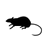
\includegraphics[width=2cm]{images/rats-module.png} \\
}
\author{
  Peter Reutemann
}

\setcounter{secnumdepth}{3}
\setcounter{tocdepth}{3}

\begin{document}

\begin{titlepage}
\maketitle

\thispagestyle{empty}
\center
\begin{table}[b]
	\begin{tabular}{c l l}
		\parbox[c][2cm]{2cm}{\copyright 2014-2018} &
		\parbox[c][2cm]{5cm}{
\includegraphics[width=5cm]{images/coat_of_arms.pdf}}
	\end{tabular}
	
\includegraphics[width=12cm]{images/cc.png} \\
\end{table}

\end{titlepage}

\tableofcontents
%\listoffigures
%\listoftables

%%%%%%%%%%%%%%%%%%%%%%%%%%%%%%%%%%%
\chapter{Introduction}
The \textit{Reception And Transmission System}, or RATS for short, is aimed
at scenarios where data is being received from various sources, processed
and then transmitted to various destinations again. It simplifies the design
of flows that handle these kind of scenarios, by providing off-the-shelf
\textit{receivers} and \textit{transmitters}, e.g., for directory polling
or FTPing files.

In contrast to regular ADAMS flows, the RATS sub-system is event-driven
and not data-driven. The received data can then be processed by a data-driven
flow before sending it somewhere else.


%%%%%%%%%%%%%%%%%%%%%%%%%%%%%%%%%%%
\chapter{Flow}
\section{Actors}
The following standalone actors are available:
\begin{itemize}
	\item \textit{Rats} -- This standalone encloses multiple RAT configurations.
	\item \textit{Rat} -- Definition of how to receive data and how to transmit 
	it, based on the specified \textit{RatInput} (= receiver) and 
	\textit{RatOutput} (= transmitter).
	\item \textit{RatPlague} -- creates copies of itself, one for each of
	the defined input queues, feeding into the same output queue.
	\item \textit{LabRat} -- the actual Rat setup gets generated at runtime
	using a generator.
\end{itemize}
The following control actors are available:
\begin{itemize}
	\item \textit{ChangeRatState} -- changes the state (eg RUNNING, PAUSED)
	of a \textit{Rat} actor. This allows the startup of Rat actors in a
	paused state before activating them later on.
	\item \textit{ExecuteRats} -- allows the execution of Rat actor(s) in
	\textit{MANUAL} mode whenever a token passes through.
\end{itemize}

%%%%%%%%%%%%%%%%%%%
% Remote commands %
%%%%%%%%%%%%%%%%%%%

\section{Remote commands}
The Rats module has some additional remote commands that allow the control of
individual \textit{Rat} actors, as long as they have been flagged to show up in a
\textit{RatControl} actor and such an actor is also present in the flow.

Available commands:
\begin{tight_itemize}
  \item \textit{flow.GetRatControlStatus} -- returns the status
  (stoppable/isstopped/pausable/ispaused) for all the registered Rat actors
  \item \textit{flow.SendRatControlCommand} -- sends the specified control command
  to a specific Rat actor (pause/resume/stop/start)
\end{tight_itemize}

%%%%%%%%%%%%%%%
% REST plugins%
%%%%%%%%%%%%%%%

\section{REST Plugins}
The following REST plugins are available:
\begin{tight_itemize}
  \item \textit{control.RatControl} -- for remote control of \textit{Rat} actors
  that show up in the \textit{RatControl} control
  panel.\footnote{adams-rats-ratcontrol\_rest\_server.flow}
  \item \textit{text.RatsTextUpload} -- for uploading raw textual
  data.\footnote{adams-rats-text\_rest\_server.flow and adams-rats-upload\_text\_via\_rest.flow}
\end{tight_itemize}

%%%%%%%%%%%%%%%%%%%%%%%%%%%%%%%%%%%
% Copyright (c) 2009-2012 by the University of Waikato, Hamilton, NZ. 
% This work is made available under the terms of the 
% Creative Commons Attribution-ShareAlike 4.0 license,
% http://creativecommons.org/licenses/by-sa/4.0/.
%
% Version: $Revision$

\begin{thebibliography}{999}
	% to make the bibliography appear in the TOC
	\addcontentsline{toc}{chapter}{Bibliography}

    % references
	\bibitem{adams}
		\textit{ADAMS} -- Advanced Data mining and Machine learning System \\
		\url{https://adams.cms.waikato.ac.nz/}{}
		
	\bibitem{heatmap}
		\textit{Heat map} -- WikiPedia article \\
		\url{http://en.wikipedia.org/wiki/Heat_map}{}

\end{thebibliography}


\end{document}
